% Settings
\documentclass[a4paper,oneside]{article}
\usepackage[slovak]{babel}
\usepackage[utf8]{inputenc}
\usepackage[pdftex]{graphicx}
\usepackage{mathtools}
\usepackage{hyperref}
\usepackage{listings}
\addtolength{\textwidth}{2cm}
\addtolength{\hoffset}{-1cm}
\addtolength{\textheight}{5cm}
\addtolength{\voffset}{-2.5cm}
% /Settings

% Content
\begin{document}

    \begin{titlepage}
        \begin{center}
            \Huge \textsc{Vysoké učení technické v Brně}\\
            \huge \textsc{Fakulta informačních technologií}\\  
            \vspace{\stretch{0.382}}
            {
\includegraphics[width=1\linewidth]{FIT_logo.pdf}} \\
            \huge \bfseries ISS projekt 2021/22\\
            \vspace{\stretch{0.618}}
        \end{center}
    
        {\large Sehnoutek Patrik (xsehno01) \hfill Brno, \today   \\}
    \end{titlepage}
    
    \tableofcontents
    \thispagestyle{empty}
    \newpage
    
    \setcounter{page}{3}

    \section{Úvod}
    Projekt som riešil pomocou skriptovacieho jazyka \textit{Python}. Na prácu so signálom som využíval knižnice \textit{numpy}, \textit{soundfile} a \textit{scipy}. Na vykreslovanie grafov som použil knižnicu \textit{matplotlib}.
    
    \section{Riešenie}
    
    % Task 4.1
    \subsection{Základy}
    
    Signál som načítal pomocou funkcie \textit{read} z knižnice \textit{soundfile}. Funkcia \textit{read} načíta už normalizovaný signál.
    \newline \newline
    \textbf{Vzorkovacia frekvencia signálu:} 16 000 Hz \\
    \textbf{Dĺžka signálu vo vzorkách:} 46695 \\
    \textbf{Dĺžka signálu v sekundách:} 2.9184375 s \\
    \textbf{Minimálna hodnota:} -0.04241943359375 \\
    \textbf{Maximálna hodnota:} 0.05169677734375 \\
    
    \begin{figure}[h]
	    \begin{center}
		    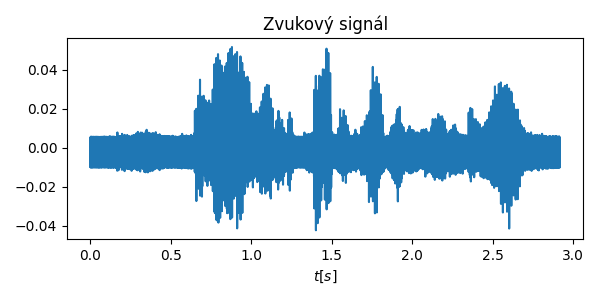
\includegraphics[width=10cm,keepaspectratio]{uloha4-1.png}
		\end{center}
	\end{figure}
	
	% Task 4.2
	\subsection{Predspracovanie rámca}
	
	Signál som si najskôr rozdelil do jednotlivých rámcov po 1024 vzorkoch, tzn. vytvoril som dvojrozmerné pole, ktoré obsahuje jednotlivé rámce. Následne som prechádzal jednotlivé rámce a hľadal rámec s periodickým charakterom.
	
	 \begin{figure}[h]
	    \begin{center}
		    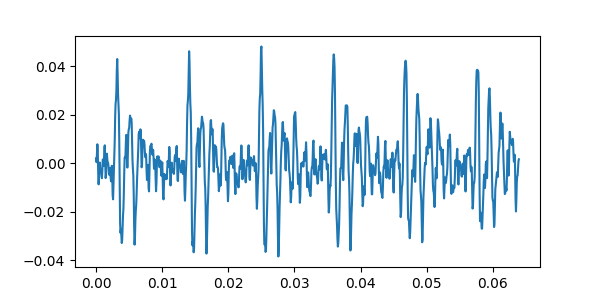
\includegraphics[width=10cm,keepaspectratio]{uloha4-2.png}
		\end{center}
	\end{figure}
	\newpage
	
	% Task 4.3
	\subsection{DFT}
	
	Na úvod som si vybral jeden z rámcov z predchádzajúcej úlohy, keďže máme pracovať s 1024 vzorkami. Následnej pomocou vlastne funkcie \textit{frame\_dft}\footnote{\url{https://pythonnumericalmethods.berkeley.edu/notebooks/chapter24.02-Discrete-Fourier-Transform.html}} aplikujem DFT na vybranom rámci. Funkcia mi vráti upravený rámec.
	
	\begin{figure}[ht]
	    \begin{center}
		    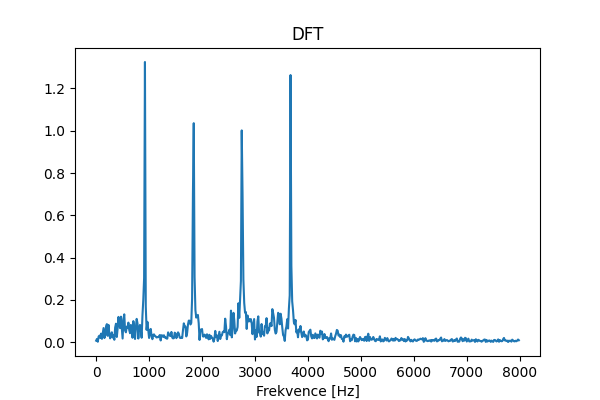
\includegraphics[width=10cm,keepaspectratio]{uloha4-3.png}
		\end{center}
	\end{figure}
	
	% Task 4.4
	\subsection{Spektogram}
	
	Na vypočítanie a zobrazenie spektorgramu som využil funkciu \textit{spectogram} z knižnice \textit{scipy.signal}. Argumentami funkcie je načítaný signál a vzorkovacia frekvencia signálu. Výstupom je pole vzorkovacích frekvencií, pole časových segmentov a spektogram signálu.
	
	\begin{center}
	       \verb|f, t, sgr = spectrogram(sig, fs)|
    \end{center}

	\begin{figure}[ht]
	    \begin{center}
		    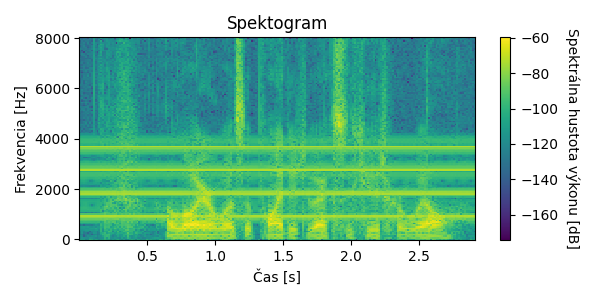
\includegraphics[width=10cm,keepaspectratio]{uloha4-4.png}
		\end{center}
	\end{figure}
	
	
	% Task 4.5
	\subsection{Určenie rušivých frekvencií}
	Rušivé frekvencie je možné vidieť aj na spektograme aj na grafe DFT. Podľa hodnôt jednotlivých frekvencií môžeme vidieť, že sú cosínusovky harmonicky vzťažené.
	
    \[f_{1}= 920Hz\ \ f_{2}= 1840Hz\ \ f_{3}= 2760Hz\ \ f_{4}= 3680 Hz\ \ \]
	
	% Task 4.6
	\subsection{Generovanie signálu}
	
	Za účelom generovaniu signálu z cosínusoviek som si vytvoril pole časových úsekov. Pole časových úsekov som použil pri vytváraní signálu z jednotlivých cosínusoviek. 
	
	\begin{center}
	        \verb|cos1 = np.cos(2 * np.pi * 920 * casove_useky)|\\
	 \end{center}
	 
	 Cosínusovky som následne spojil do jedného signálu. Výsledný signál som vygeneroval pomocou funkcie \textit{wavfile.write}.
	 
	 \begin{center}
	 \verb|wavfile.write("audio/4cos.wav", fs, cos_merge.astype(np.float32))|
    \end{center}
	
	\begin{figure}[h]
	    \begin{center}
		    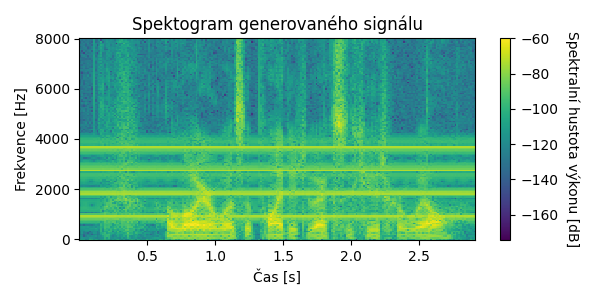
\includegraphics[width=10cm,keepaspectratio]{uloha4-6.png}
		\end{center}
	\end{figure}
	
	
	% Task 4.7
	\subsection{Čistiaci filter}
	
	Čistiace filtre som vytvoril pomocou funkcie \textit{scipy.signal.butter}. Zvolil som si zo zadania metódu č.3, návrh 4 pásmových zádrží. 
	
	\begin{center}
	       \verb|b1, a1 = butter(4, [low, high], btype="bandstop")|
    \end{center}
	
	\begin{figure}[h]
	    \begin{center}
		    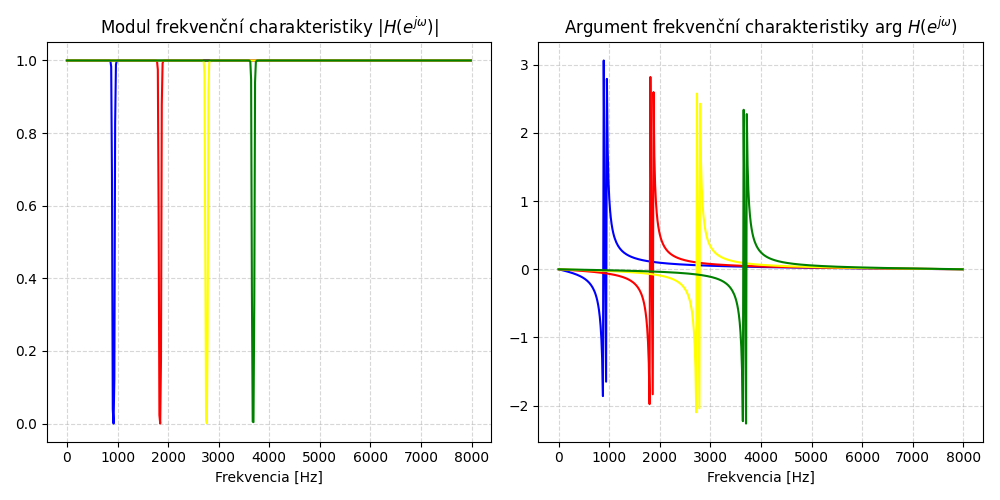
\includegraphics[width=12cm,keepaspectratio]{uloha4-7.png}
		\end{center}
	\end{figure}
	
	Pre zobrazenie impulzných odoziev som zvolil 50 vzorkov. Kedže ide o IIR filtre je potrebné ich obmedziť na dĺžku vhodnú na zobrazenie. \\
	
	\textbf{Koeficienty filtrov:}
	\begin{center}
	    \verb|b_1 = [  0.96968306  -7.25717748  24.24619573 -47.17679161  58.43644899 -47.17679161|
	    \verb|24.24619573  -7.25717748   0.96968306]|
    	\verb|a_1 = [  1.          -7.42647266  24.62102491 -47.53815186  58.4323126 -46.81199214|
    	\verb|23.87458382  -7.09132154   0.94028524]|
        \verb|b_2 = [  0.96968306  -5.81936384  16.97514878 -30.55735654  36.92422423 -30.55735654|
        \verb|16.97514878  -5.81936384   0.96968306]|
        \verb|a_2 = [  1.          -5.95511774  17.23747829 -30.79114816  36.92123644 -30.32080708|
        \verb|16.71488794  -5.68636777   0.94028524]|
        \verb|b_3 = [  0.96968306  -3.63020085   8.97512354 -14.07049444  16.7549157 -14.07049444|
        \verb|8.97512354  -3.63020085   0.96968306]|
        \verb|a_3 = [  1.          -3.71488604   9.11367444 -14.17791825  16.75319166 -13.96135026|
        \verb|8.83737757  -3.54723603   0.94028524]|
        \verb|b_4 = [ 0.96968306 -0.97233559  4.24435552 -2.97811066  6.55317435 -2.97811066|
        \verb|4.24435552 -0.97233559  0.96968306]|
        \verb|a_4 = [ 1.         -0.9950182   4.30971065 -3.00079861  6.55219762 -2.95496191|
        \verb|4.179058   -0.95011377  0.94028524]|
    \end{center}

	
	% Task 4.8
	\subsection{Nulové body a póly}
	
	Nulové body a póly som získal z filtrov pomocou funkcie \textit{scipy.signal.butter} s výstupom \textit{zpk}. Následne som nulové body a póly zo všetkých filtrov zobrazil na jednu jednotkové kružnicu.
	
	\begin{center}
	        \verb|z1, p1, k1 = butter(4, [low, high], btype="bandstop", output="zpk")|
    \end{center}
	
	\begin{figure}[h]
	    \begin{center}
		    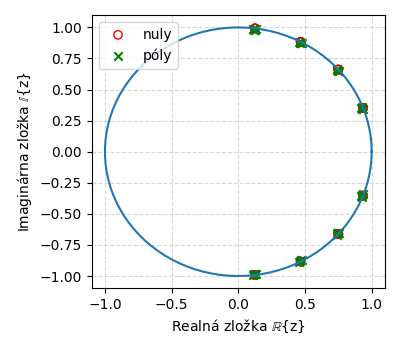
\includegraphics[width=6cm,keepaspectratio]{uloha4-8.png}
		\end{center}
	\end{figure}
	
	%filtre
	%https://docs.scipy.org/doc/scipy/reference/generated/scipy.signal.butter.html
	
	% Task 4.9
	\subsection{Frekvenčná charakteristika}
	
	Frekvenčnú charakteristiku som realizoval pomocou funkcie \textit{scipy.signal.freqz} postupne pre každý filter.
	
	\begin{center}
	        \verb|freq1, h1 = freqz(b1, a1)|
    \end{center}
	
	\begin{figure}[h]
	    \begin{center}
		    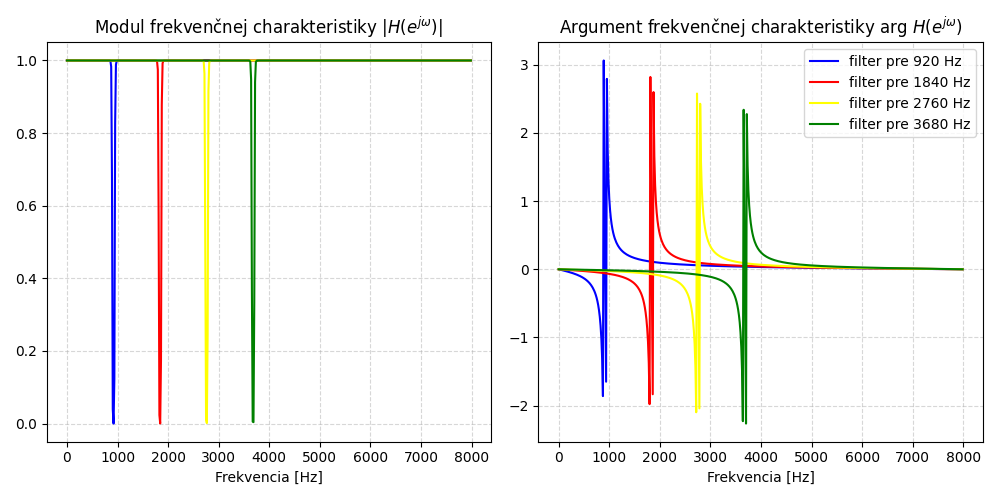
\includegraphics[width=12cm,keepaspectratio]{uloha4-9.png}
		\end{center}
	\end{figure}
	
	% Task 4.10
	\newpage
	\subsection{Filtrácia}
	
	Signál som vyfiltroval pomocou funkcie \textit{scipy.signal.lfilter} so všetkými 4 navrhnutými filtrami. Filtrovaný signál je vyčistený, avšak na začiatku signálu sa objavil artefakt. Je to spôsobené tým, že aj filter má nejakú impulznú odovzvu. Prvých pár vzorkov sa bude správať inak, tzn. na výstup sa prekopírujú vzorky z pôvodného signálu.
	
	\begin{figure}[h]
	    \begin{center}
		    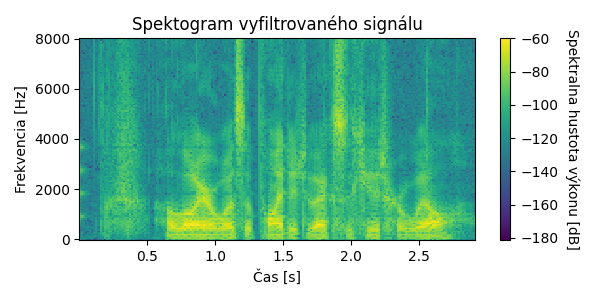
\includegraphics[width=10cm,keepaspectratio]{uloha4-10-1.png}
		    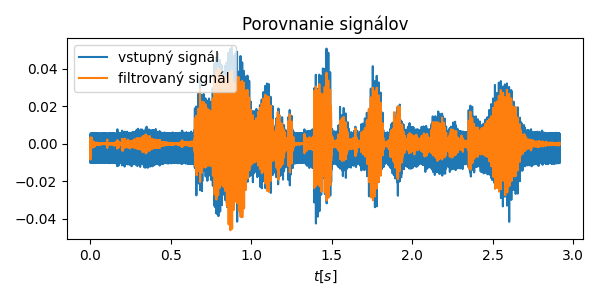
\includegraphics[width=10cm,keepaspectratio]{uloha4-10-2.png}
		\end{center}
	\end{figure}
    
    Podľa spektogramu a vypočutia si výsledného zvuku usudzujem, že som rušivé frekvencie úspešne odstránil a splnil zadanie projektu.

\end{document}
